
\section{Study of Parallel Workload \Rmnum{2 }}
%\section{``Bully" become ``bullied"}
\label{sec:workload-2}

In this section, we use a different experimental configuration to verify and
explore the observations made in the previous section. Specifically, we conduct
the same sets of experiments through Workload~\Rmnum{2}, which consists of sAMG,
MultiGrid and CrystalRouter.
%\NOTE{By replacing AMG with sAMG, we turn the ``bully" into the ``bullied".} 
The ``bully" becomes the ``bullied" with the presence of sAMG in Workload~\Rmnum{2}. 


\subsection{Network Performance Analysis}
\label{sec: workload-2 network analysis}

Figure~\ref{fig:synwkld-network-traffic-stime} shows aggregate traffic and
saturation times for Workload~\Rmnum{2}, corresponding to
Figure~\ref{fig:wkld-network-traffic-stime} in Workload~\Rmnum{1}. Replacing
AMG with sAMG results in greater aggregate traffic as well as more saturation
than in Workload~\Rmnum{1}, but regardless, similar patterns can be observed.
Contiguous placement with minimal routing results in load imbalance with
respect to both traffic and saturation. The addition of adaptive routing
alleviates these effects to some degree, particularly with respect to global
channel usage, while trading off saturation in global channels for saturation in
the local channels. Using random placement again shows roughly similar performance
characteristics across routing configurations, with adaptive routing helping to
balance aggregate load while increasing the aggregate traffic due to the related
indirection.

\begin{figure*}[t]
    \centering
    \begin{subfigure}[t]{0.32\textwidth}
        \centering
        \includegraphics[height=1.5 in]{syn-wkld/gc-traffic}
        \caption{Global Channel Traffic}
        \label{fig:synwkld-global-channel-traffic}
    \end{subfigure}\hfill
    \hspace{1em}%
    \begin{subfigure}[t]{0.32\textwidth}
        \centering
        \includegraphics[height=1.5 in]{syn-wkld/lc-traffic}
        \caption{Local Channel Traffic}
        \label{fig:synwkld-local-channel-traffic}
    \end{subfigure}\hfill
    \hspace{1em}%
    \begin{subfigure}[t]{0.32\textwidth}
        \centering
        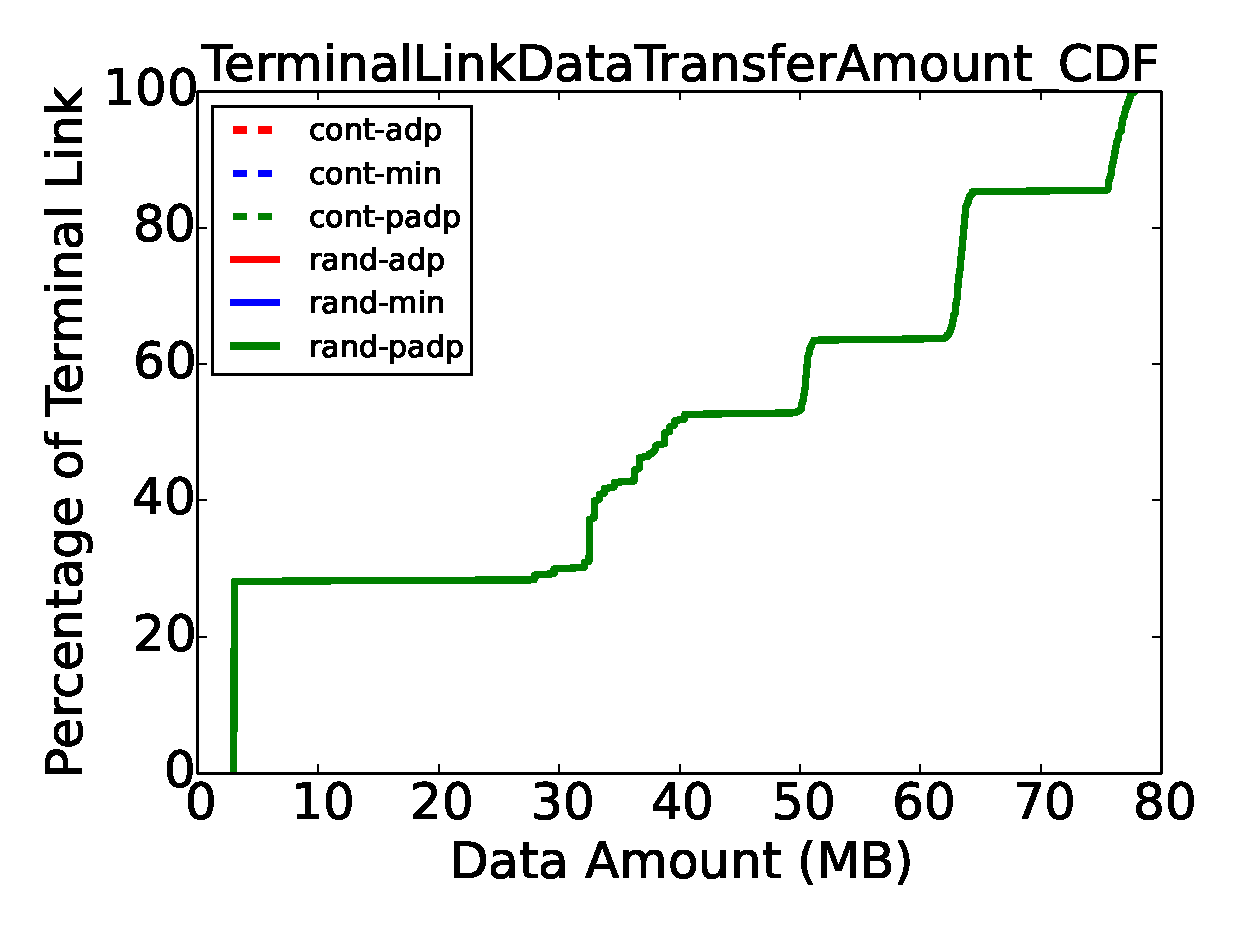
\includegraphics[height=1.5 in]{syn-wkld/tl-traffic}
        \caption{Terminal Link Traffic}
        \label{fig:synwkld-terminal-link-traffic}
    \end{subfigure}\\

    \begin{subfigure}[t]{0.32\textwidth}
        \centering
        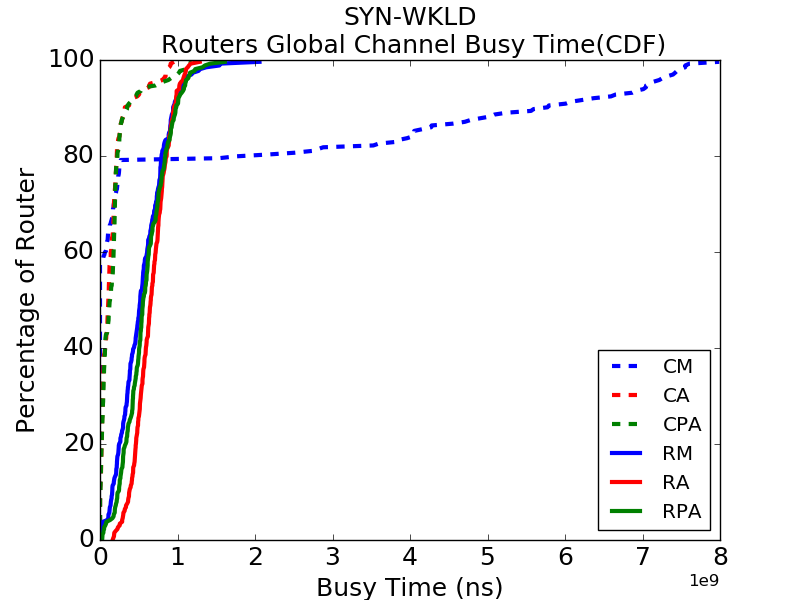
\includegraphics[height=1.5 in]{syn-wkld/gc-btime}
        \caption{Global Channel Saturation Time}
        \label{fig:synwkld-global-channel-stime}
    \end{subfigure}\hfill
     \hspace{1em}%
    \begin{subfigure}[t]{0.32\textwidth}
        \centering
        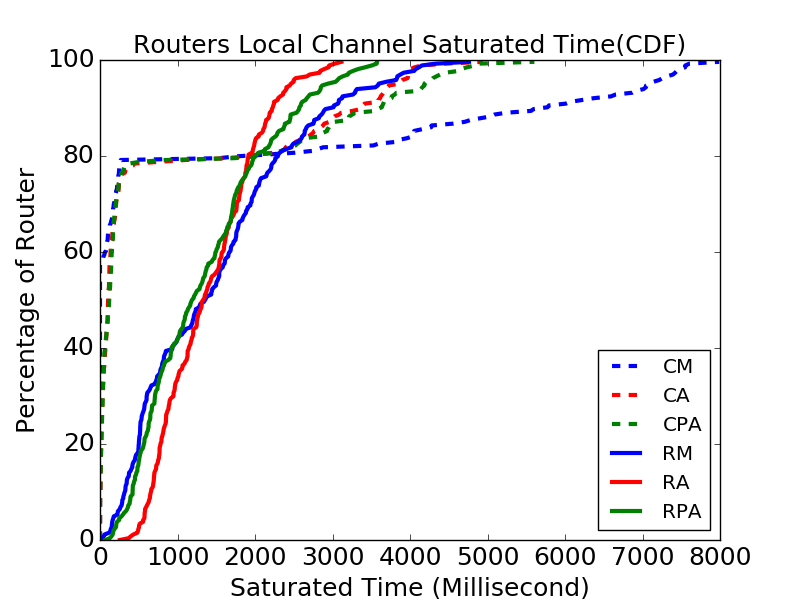
\includegraphics[height=1.5 in]{syn-wkld/lc-btime}
        \caption{Local Channel Saturation Time}
        \label{fig:synwkld-local-channel-stime}
    \end{subfigure}\hfill
    \hspace{1em}%
    \begin{subfigure}[t]{0.32\textwidth}
        \centering
        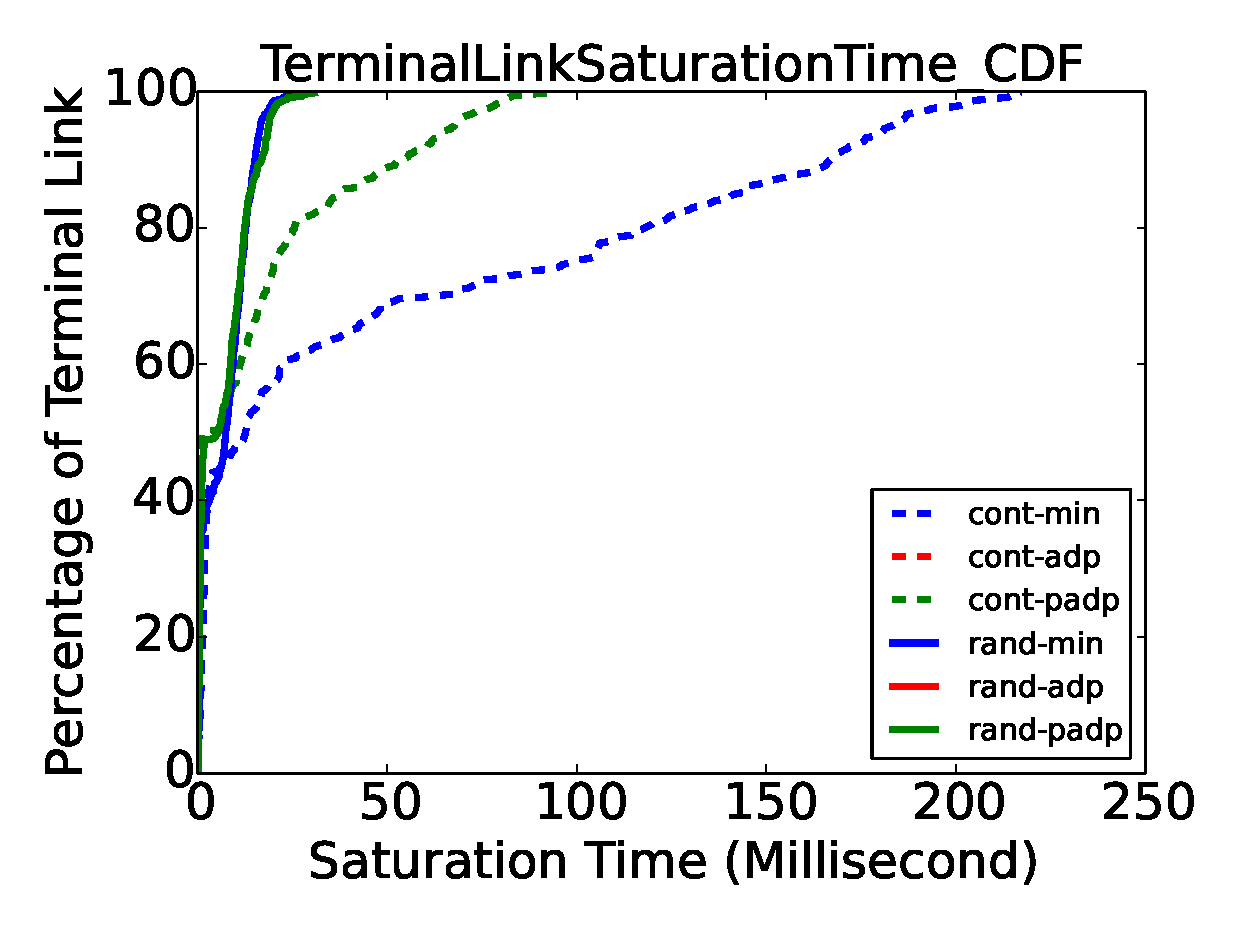
\includegraphics[height=1.5 in]{syn-wkld/tl-btime}
        \caption{Terminal Link Saturation Time}
        \label{fig:synwkld-terminal-link-stime}
    \end{subfigure}%
   \caption{Aggregate traffic and saturation time for Workload~\Rmnum{2} under the configurations listed in Table~\ref{tab: placement routing configs}. For either contiguous or random placement, ``adp'' and ``padp'' have equivalent behavior.}
   \label{fig:synwkld-network-traffic-stime}
\end{figure*}


%+================================================================
%The average communication time spent by all MPI ranks when Workload~\Rmnum{2} is running under different placement and routing configurations shown in Table~\ref{tab:syn-wkld-commtime}. 
%We can observe the similar pattern as in Table~\ref{tab:wkld-commtime}
%The contiguous placement coupled with minimal routing results in highest communication time. 
%The random placement coupled with minimal routing is the most efficient. 
%Progressive adaptive routing is better than adaptive routing when random placement is in use, 
%and they have comparable results when coupled contiguous placement. 
%Same as Workload~\Rmnum{1}, the network reaches the optimal performance when Workload~\Rmnum{2} is running with random placement and adaptive routing. 
%
%\begin{table}[ht]
%\begin{center}
%\caption{Average time spent on communication by all MPI ranks when Workload II is running on dragonfly network under six different placement and routing configurations.} 
%\label{tab:syn-wkld-commtime}
%%\centering % Centers the table on the page, comment out to left-justify
%\begin{tabular}{l c c c c c c }
%\toprule % Top horizontal line
%\toprule
%&\multicolumn{6}{c}{Placement and Routing Configuration} \\ % Amalgamating several columns into one cell is done using the \multicolumn command as seen on this line
%\cmidrule(l){2-7}
%          & CM & CA & CPA & RM & RA & RPA \\ % Column names row
%\midrule % In-table horizontal line
%Time(ms)  & 3360 & 2204 & 2335 & 1791 & 2367 & 1965 \\ % Content row 1
%
%\midrule % In-table horizontal line
%\bottomrule % Bottom horizontal line
%\end{tabular}
%\end{center}
%\end{table}



\subsection{Individual Application Analysis}
\label{sec: workload-2 app analysis}

We study the performance of each application individually in the same manner as
in Section~\ref{sec: workload-1 app analysis}.
Figure~\ref{fig:syn-apps-commtime} shows the communication time distributions of
the ranks of the three applications, running concurrently in Workload~\Rmnum{2}.
The ``bully" in Workload~\Rmnum{1} becomes the ``bullied" in Workload~\Rmnum{2}. 
MultiGrid and CrystalRouter are in this instance the less communication-intensive applications. 
With random placement and (progressive) adaptive routing, 
both MultiGrid and CrystalRouter experience prolonged communication time, 
as shown in Figure~\ref{fig:syn-mg-commtime}, \ref{fig:syn-cr-commtime}. 
On the other hand, sAMG (Figure~\ref{fig:syn-samg-commtime}) benefits from those configurations
in a similar manner to CrystalRouter in Workload~\Rmnum{1}.
Contiguous placement coupled with minimal routing, while preventing the ``bully"
behavior, results in poor performance for all of the applications except CrystalRouter,
which we expect is due to a higher degree of network isolation.

\begin{figure*}[t!]
    \centering
    \begin{subfigure}[t]{0.32\textwidth}
        \centering
        \includegraphics[height=1.5 in]{syn-wkld/mg/commtime}
        \caption{MultiGrid}
        \label{fig:syn-mg-commtime}
    \end{subfigure}%
    \hspace{1em}%
    \begin{subfigure}[t]{0.32\textwidth}
        \centering
        \includegraphics[height=1.5 in]{syn-wkld/cr/commtime}
        \caption{CrystalRouter}
        \label{fig:syn-cr-commtime}
    \end{subfigure}%
    \hspace{1em}%
    \begin{subfigure}[t]{0.32\textwidth}
        \centering
        \includegraphics[height=1.5 in]{syn-wkld/amg10/commtime}
        \caption{sAMG}
        \label{fig:syn-samg-commtime}
    \end{subfigure}%
    \caption{Communication time distribution across application ranks in Workload~\Rmnum{2}. The ``bully", sAMG, benefits from random placement and adaptive routing, while the ``bullied", MultiGrid and CrystalRouter, suffer performance degradation.}
   \label{fig:syn-apps-commtime}
\end{figure*}



% explain the network status of sAMG, MG and CR
Once again, we look at the network-level system view to scrutinize the traffic through the routers serving each application. 
The routers serving sAMG have a high volume of traffic on both local and global channels when contiguous placement is in use, 
as shown in Figures~\ref{fig:syn-samg-lc-traffic} and \ref{fig:syn-samg-gc-traffic}.
As in previous results, the use of random placement alleviates the local congestion by uniformly distributing the traffic of sAMG over the network, getting more routers involved in serving sAMG.
In this case, a majority of those less busy routers are also serving MultiGrid and CrystalRouter.



%MultiGrid and CrystalRouter are the less communication-intensive applications in Workload~\Rmnum{2}.
% JJ - I shortened this
%When MultiGrid is running with contiguous placement, the serving routers have a comparatively small volume of traffic on their local and global channels, as shown in Figure~\ref{fig:syn-mg-lc-traffic} and \ref{fig:syn-mg-gc-traffic}. When coupled with (progressive) adaptive routing, more MultiGrid traffic traverses global channels, while more aggregate traffic is seen on the local channels due to the additional intermediate hops.
%When random placement is in use, the MPI ranks of MultiGrid are randomly distributed across the network and share routers with other applications. The routers serving MultiGrid have much more traffic on their local and global channels, as shown in Figures~\ref{fig:syn-mg-lc-traffic} and \ref{fig:syn-mg-gc-traffic}. The increased traffic comes largely from sAMG. \TODO{can shorten this}

MultiGrid in Workload~\Rmnum{2} is similar to AMG in Workload~\Rmnum{1} when considering resident channel behavior, as shown in Figures~\ref{fig:syn-mg-lc-traffic} and \ref{fig:syn-mg-gc-traffic}. There is a large gap in traffic volume between the contiguous and random placement approaches, due to other applications (sAMG in particular) utilizing the same links. CrystalRouter in Workload~\Rmnum{2} additionally experiences more load on its channels using random allocation configurations, as shown in Figure~\ref{fig:syn-cr-lc-traffic} and \ref{fig:syn-cr-lc-traffic}. However, the maximal load under random allocation is closer to that observed in contiguous allocations as compared to MultiGrid.

\begin{figure*}[t]
    \centering
    \begin{subfigure}[t]{0.32\textwidth}
        \centering
        \includegraphics[height=1.5 in]{syn-wkld/mg/lc-traffic}
        \caption{MultiGrid Local Channel Traffic}
        \label{fig:syn-mg-lc-traffic}
    \end{subfigure}\hfill
    \begin{subfigure}[t]{0.32\textwidth}
        \centering
        \includegraphics[height=1.5 in]{syn-wkld/cr/lc-traffic}
        \caption{CrystalRouter Local Channel Traffic}
        \label{fig:syn-cr-lc-traffic}
    \end{subfigure}\hfill
    \begin{subfigure}[t]{0.32\textwidth}
        \centering
        \includegraphics[height=1.5 in]{syn-wkld/amg10/lc-traffic}
        \caption{sAMG Local Channel Traffic}
        \label{fig:syn-samg-lc-traffic}
    \end{subfigure}\\
    \centering
    \begin{subfigure}[t]{0.32\textwidth}
        \centering
        \includegraphics[height=1.5 in]{syn-wkld/mg/gc-traffic}
        \caption{MultiGrid Global Channel Traffic}
        \label{fig:syn-mg-gc-traffic}
    \end{subfigure}\hfill
    \begin{subfigure}[t]{0.32\textwidth}
        \centering
        \includegraphics[height=1.5 in]{syn-wkld/cr/gc-traffic}
        \caption{CrystalRouter Global Channel Traffic}
        \label{fig:syn-cr-gc-traffic}
    \end{subfigure}\hfill
    \begin{subfigure}[t]{0.32\textwidth}
        \centering
        \includegraphics[height=1.5 in]{syn-wkld/amg10/gc-traffic}
        \caption{sAMG Global Channel Traffic}
        \label{fig:syn-samg-gc-traffic}
    \end{subfigure}
    \caption{Aggregate workload traffic for routers serving specific applications. More routers are involved in serving each application when random placement is in use, compared to contiguous placement. For either contiguous or random placement, ``adp'' and ``padp'' have equivalent behavior.}
   \label{fig:syn-3app-gc-traffic}
\end{figure*}



\subsection{Key Observations}

%\NOTE{rewrote this somewhat. The observations made were essentially the same as the previous section}

Revisiting the observations in Section~\ref{sec:workload-1-observations}, we
find that those observations are held under this separate configuration.
%System-level performance is still much improved in terms of load-balancing.
System-level performance is still much improved in terms of load-balancing with random placement.
sAMG, being far and away the most communication-intensive application in Workload~\Rmnum{2}, benefits
greatly from random placement, whereas in Workload~\Rmnum{1} AMG was effectively
penalized for being less communication-intensive. CrystalRouter, being the
comparatively less communication-intensive application in Workload~\Rmnum{2},
experiences performance regressions in Workload~\Rmnum{2} under random and adaptive
policies.

Interestingly, in both Workload~\Rmnum{1} and \Rmnum{2}, MultiGrid experiences
a more subtle performance variatioin than the significant swings in performance
observed in the other applications. These behaviors persisted across multiple runs
with different random seeds. Additionally, CrystalRouter in Workload~\Rmnum{2}
has less drastic changes in maximal load, but still experiences performance
regressions. We are continuing to work towards understanding the root causes
and implications of this behavior, for which we expect application-specific
communication patterns to be an important factor. 
%\TODO{Is this a reasonable observation? Yes, it is.}
